\documentclass[11pt,titlepage]{article}
\usepackage[utf8]{inputenc}
\usepackage[dutch]{babel}
\usepackage{amsmath}
\usepackage{amsfonts}
\usepackage{amssymb}
\usepackage{graphicx}
\usepackage[table,xcdraw]{xcolor}
\usepackage[toc,page]{appendix}
\usepackage{hyperref}
\usepackage{listings}
\usepackage{float}
\usepackage{tikz}
\usetikzlibrary{trees}
\usepackage{tikz-qtree}
\usepackage{graphicx}
\usepackage{fancyref}
\usepackage{wrapfig}
\usepackage{url}
\usepackage{pdflscape}
\usepackage{fancyvrb}
\graphicspath{ {Afbeeldingen/} }
\usepackage{subfig}
\usepackage{tabularx}

\newcolumntype{L}[1]{>{\raggedright\arraybackslash}p{#1}}

%% Sets page size and margins 
\usepackage[a4paper,top=3cm,bottom=3cm,left=3cm,right=3cm,marginparwidth=1.75cm]{geometry}

\author{René van Eendenburg 561378 \cr Derk Wiegerinck 567665}

\title{Ontwerp Documentatie}
\usepackage{titling}

\newcommand{\subtitle}[3]{%
	\posttitle{%
		\par\end{center}
	\begin{center}\large#1\end{center}
	\begin{center}\large#2\end{center}
	\begin{center}\large#3\end{center}
	\vskip0.5em}%
}

\subtitle{HAN Arnhem}{Versie 1}{WOR-World}

\frenchspacing
\sloppy
\begin{document}
\maketitle



\tableofcontents
\clearpage


\section{Inleiding}
Dit document bevat het ontwerp van de simulatie opdracht. Hier zal worden ingegaan op de structuur van de packages, samenhang van de broncode en 

\section{Structuur}

\subsection{al5d\_simulation}
De al5d\_simulation package bevat een programma die de al5d controller simuleert en de visualisatie van de lynxmotion al5d.\newline 
\newline
De controller accepteert berichten van het \href{https://www.robotshop.com/media/files/pdf2/lynxmotion_ssc-32u_usb_user_guide.pdf
}{SSC32U} format op een rostopic. Het rostopic, genaamd "SSC32U\_request\_topic", handelt alle mogelijke requests af. Responses zijn op dit moment niet geïmplementeerd omdat dit buiten de scope van de opdracht ligt.\newline
Bij een request zal de al5d\_simulation de SSC32U requests converteren en vervolgens publiceren op het "joint\_state\_message\_topic". Deze worden op hun beurt weer afgehandeld door de "robot\_state\_publisher". Dit topic zal de robot in de Rviz visualisatie aansturen.

\subsection{cup}
De cup package bevat een programma die bekers kan simuleren. Deze package maakt gebruik aanwezige transforms binnen de simulatie. Dit gebeurd door middel van een TransformListener. Er wordt geluisterd naar de locatie van de grippers om daarmee te bepalen of het bekertje is opgepakt of is losgelaten. Daarnaast kijkt de beker naar zijn eigen locatie of er zwaartekracht uitgeoefend wordt op de beker.
\newline
De beker maakt ook gebruik van "visualization msgs" om zichzelf te laten weergeven in de simulatie als een marker. Deze messages worden gepubliceerd op het topic "visualization marker".
\newline
Om een beker in de simulatie wereld te weergeven, moeten de volgende argumenten worden meegegeven. Een numeriek ID, X locatie, Y locatie en een Z locatie. 

\section{Realisatie}

\subsection{al5d\_simulation}

De al5d is opgezet in de volgende onderdelen. Een command parser, servo aansturing, een publisher en een controller klasse. Na het klassediagram zal er een kleine beschrijving van elk onderdeel staan.

\begin{figure}[H]
\centering
    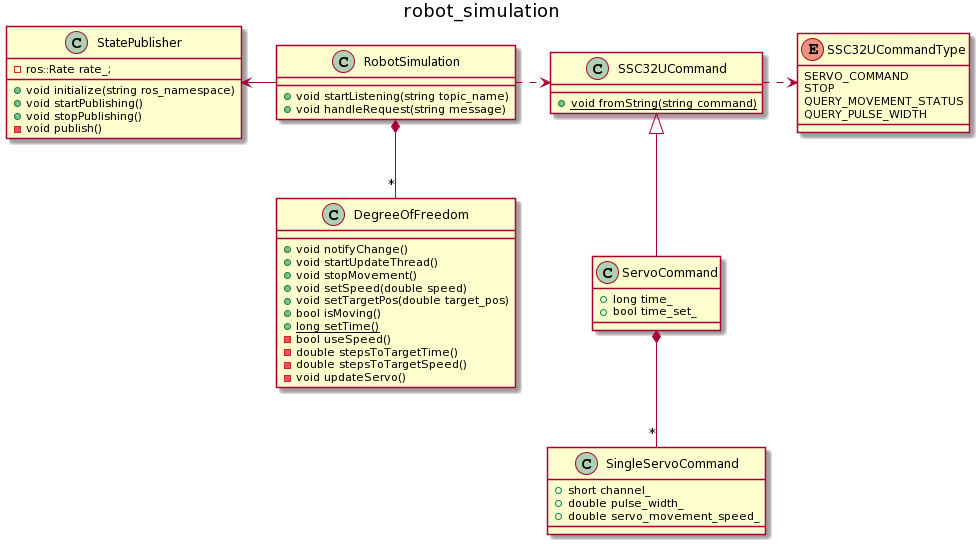
\includegraphics[scale = .4]{robot_sim_plantuml.png}
    \caption{al5d\_simulation class diagram}
    \label{figure:al5d_simulation}
\end{figure}

\subsubsection{SSC32UCommand}
Deze klasse parsed SSC32U string commando's en geeft een SSC32U object terug. Dit object kan een ServoCommand zijn, deze kan meerdere SingleServoCommands bevatten. Hierin zitten het kanaal voor de servo, de gewenste positie en de snelheid voor de servo. In een ServoCommand kan ook een globale tijd worden gezet. De keus voor individuele servo snelheid of de globale tijd wordt gebruikt, wordt afgehandeld in DegreeOfFreedom.

\subsubsection{DegreeOfFreedom}
Een object van deze klasse dient als een enkele servo. De servo ontvangt een target positie waar de servo naar toe moet bewegen. De servo zal vervolgens berekenen, op basis van de gegeven snelheid, tijd of limitaties van de servo, in hoe veel stappen er bewogen wordt naar de target positie. De limitaties van de servo worden opgehaald van de Ros Parameter server. Deze parameter server wordt geladen met een xarco file.

\subsubsection{StatePublisher}
Deze klasse benodigd een lijst met alle servo's. Vervolgens zal deze met een vaste rate door de lijst heen loopen in de functie Publish en daarmee de configuratie van de robot arm doorsturen naar het "joint\_state\_message\_topic".

\subsubsection{RobotSimulation}
De RobotSimulation is de controller van de al5d\_simulation. Deze handelt de requests af die binnen komen op het rostopic.


\end{document}
